\documentclass{beamer}
\usepackage[spanish]{babel}
\usetheme{metropolis}           % Use metropolis theme
\graphicspath{{images/}}

\usepackage{multicol}
\usepackage{listings}
\usepackage[default]{sourcesanspro}

\usepackage[scale=2]{ccicons}



\lstdefinestyle{eisvogel_listing_style}{
  language         = c++,
%$if(listings-disable-line-numbers)$
%  xleftmargin      = 0.6em,
%  framexleftmargin = 0.4em,
%$else$
  numbers          = left,
  xleftmargin      = 0em,
 framexleftmargin = 0em,
%$endif$
  breaklines       = true,
  frame            = single,
    tabsize          = 2,
  literate         =
  {á}{{\'a}}1 {é}{{\'e}}1 {í}{{\'i}}1 {ó}{{\'o}}1 {ú}{{\'u}}1
  {Á}{{\'A}}1 {É}{{\'E}}1 {Í}{{\'I}}1 {Ó}{{\'O}}1 {Ú}{{\'U}}1
  {à}{{\`a}}1 {è}{{\'e}}1 {ì}{{\`i}}1 {ò}{{\`o}}1 {ù}{{\`u}}1
  {À}{{\`A}}1 {È}{{\'E}}1 {Ì}{{\`I}}1 {Ò}{{\`O}}1 {Ù}{{\`U}}1
  {ä}{{\"a}}1 {ë}{{\"e}}1 {ï}{{\"i}}1 {ö}{{\"o}}1 {ü}{{\"u}}1
  {Ä}{{\"A}}1 {Ë}{{\"E}}1 {Ï}{{\"I}}1 {Ö}{{\"O}}1 {Ü}{{\"U}}1
  {â}{{\^a}}1 {ê}{{\^e}}1 {î}{{\^i}}1 {ô}{{\^o}}1 {û}{{\^u}}1
  {Â}{{\^A}}1 {Ê}{{\^E}}1 {Î}{{\^I}}1 {Ô}{{\^O}}1 {Û}{{\^U}}1
  {œ}{{\oe}}1 {Œ}{{\OE}}1 {æ}{{\ae}}1 {Æ}{{\AE}}1 {ß}{{\ss}}1
  {ç}{{\c c}}1 {Ç}{{\c C}}1 {ø}{{\o}}1 {å}{{\r a}}1 {Å}{{\r A}}1
  {€}{{\EUR}}1 {£}{{\pounds}}1 {«}{{\guillemotleft}}1
  {»}{{\guillemotright}}1 {ñ}{{\~n}}1 {Ñ}{{\~N}}1 {¿}{{?`}}1
  {…}{{\ldots}}1 {≥}{{>=}}1 {≤}{{<=}}1 {„}{{\glqq}}1 {“}{{\grqq}}1
  {”}{{''}}1}
\lstset{style=eisvogel_listing_style}




\hypersetup{
    colorlinks=true,
    linkcolor=black,
    filecolor=magenta,
    urlcolor=cyan,
}

\title{MH: Práctica 4\\
			PAR - Estudio y propuesta de metaheurística propia}


\date{\today}
\author{Antonio David Villegas Yeguas}
\institute{Universidad de Granada\\
\medskip
\textit{advy99@correo.ugr.es}
}
\setbeamertemplate{caption}{\raggedright\insertcaption\par}

\begin{document}

 \maketitle

\begin{frame}{Índice}
\tableofcontents
\end{frame}
  
  
\section{Inspiración}
\begin{frame}{Inspiración: Filosofía de Nietzsche}

	\begin{minipage}{0.3\textwidth}
    	\begin{figure}
   		 	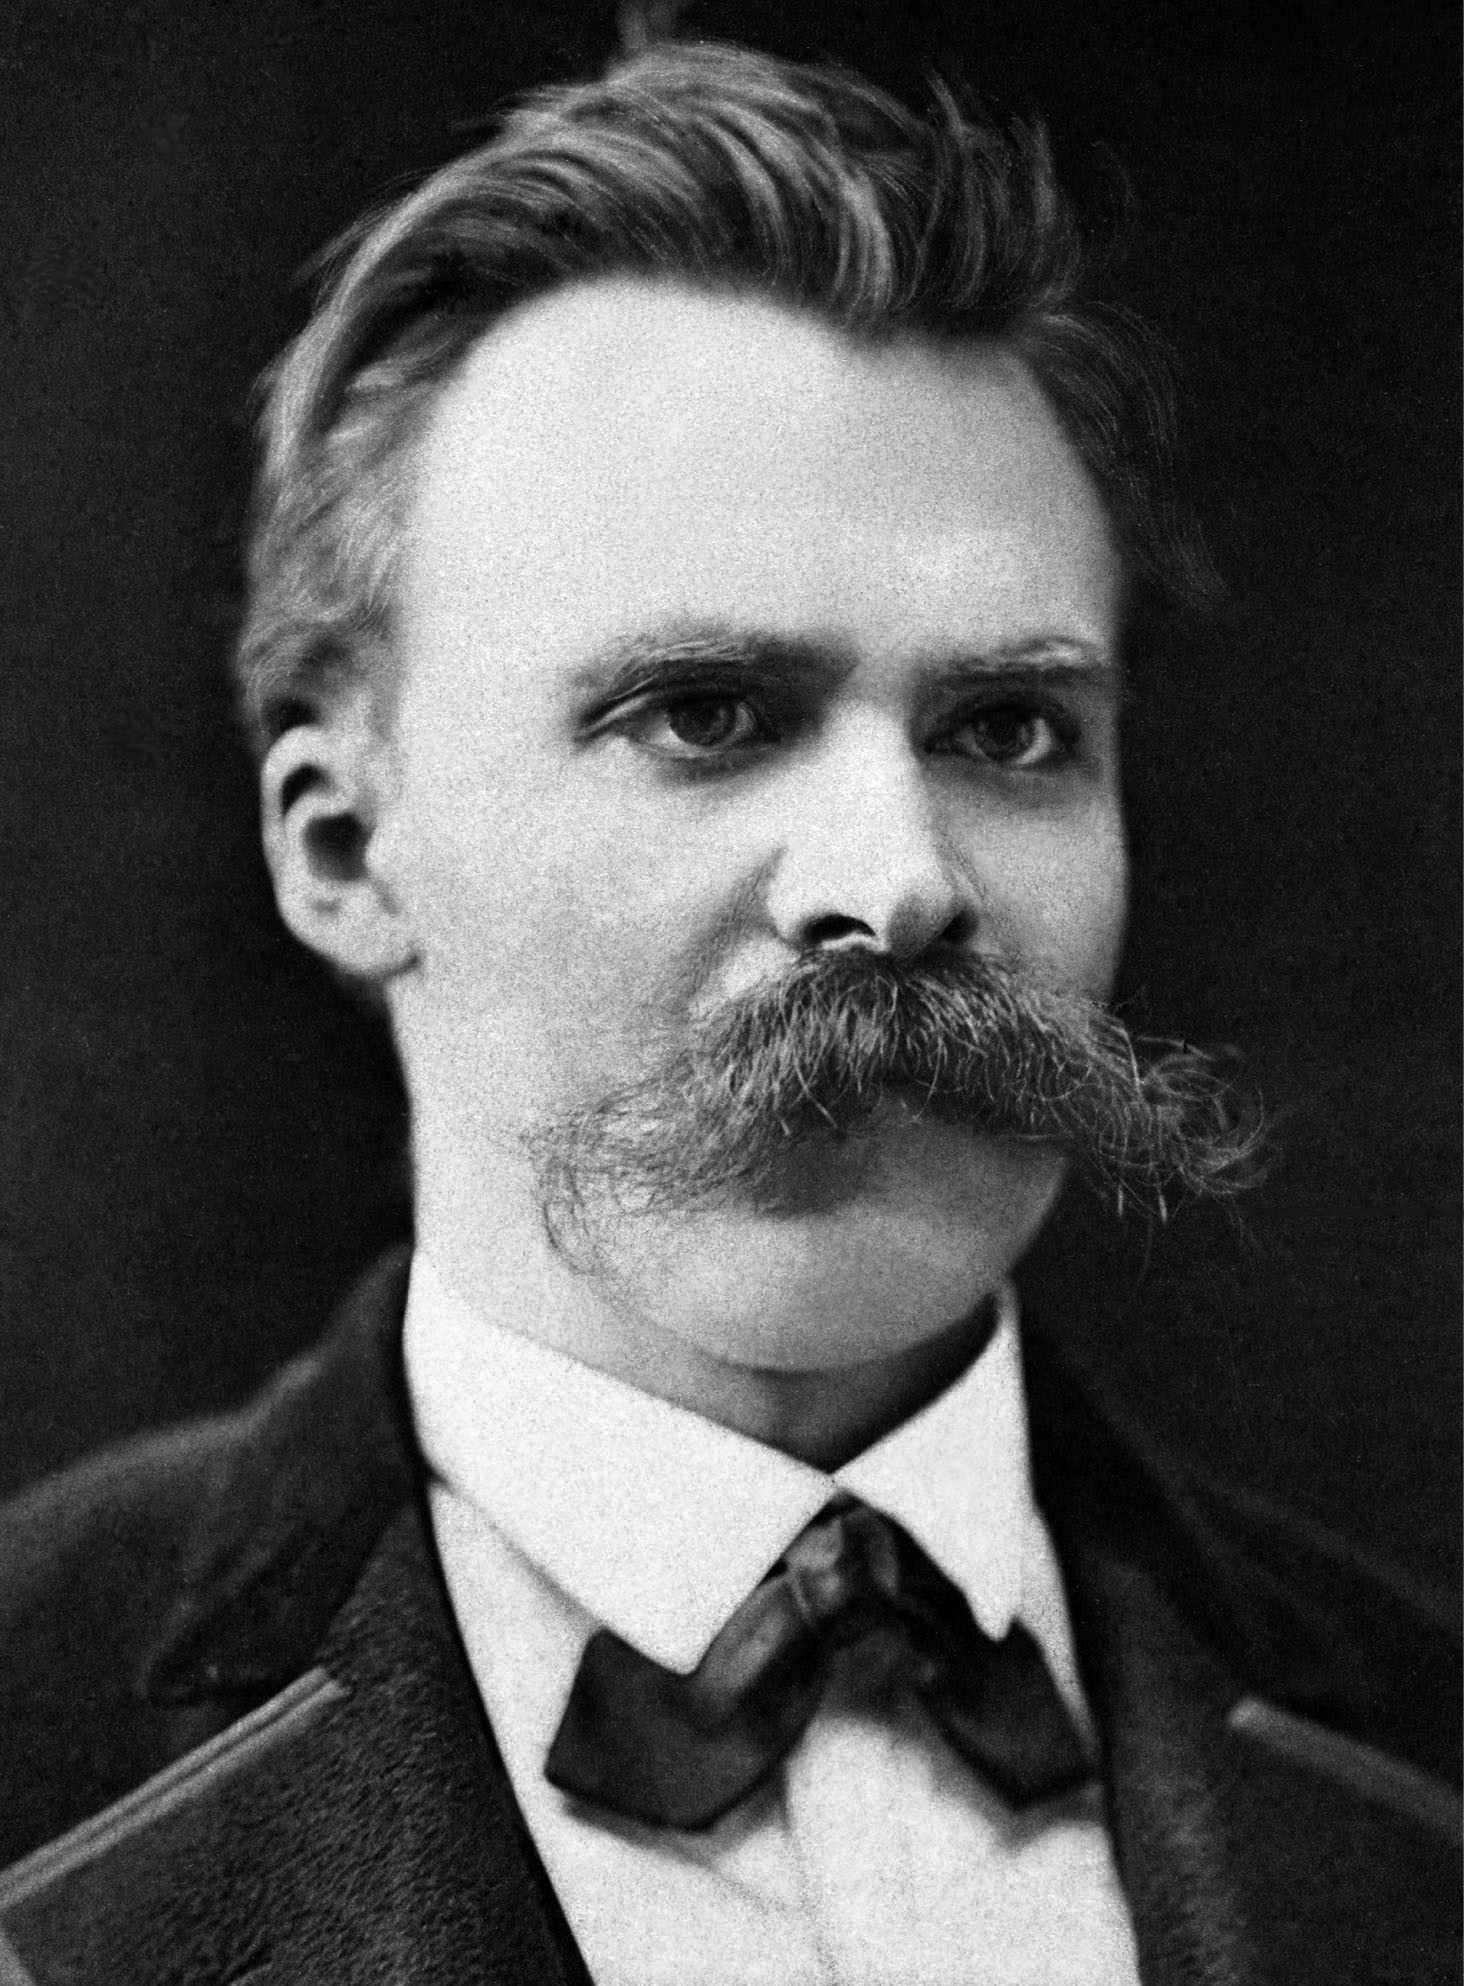
\includegraphics[scale=0.26]{nietzsche.jpg}
    		\caption{\footnotesize{Friedrich Nietzsche 15/10/1844 - 25/09/1900}}
   	
    	\end{figure}
    	
    \end{minipage}
    \hfill
	\begin{minipage}{0.65\textwidth}	
    	Idea obtenida de la filosofía de Nietzsche:
    
    	\begin{itemize}
			\item Sociedad sumida en nihilismo existencial. Desvalorización de los valores morales.
			\item Búsqueda del superhombre. Ser superior capaz de crear una moral propia, nuevos valores morales.
    	\end{itemize}
	\end{minipage}
	
\end{frame}
  
  
  
\section{Propuesta}
  
\begin{frame}{Propuesta: Dos poblaciones}
Siguiendo la idea de Nietzsche, algoritmo con dos poblaciones:

\begin{enumerate}
	\item Población con superhombre:
		\begin{itemize}
			\item Explotación del entorno. 
			\item La mejor solución hará de superhombre.
			\item El resto de soluciones intentarán parecerse a esta solución.
		\end{itemize}
	\item Población sumida en el nihilismo: 
		\begin{itemize}
			\item Exploración del entorno.
			\item Búsqueda de mejores zonas del espacio de búsqueda. 
			\item No creen en los valores morales del superhombre, las soluciones de esta población intentarán ser distintas a la mejor solución. Intentar salir del nihilismo.
		\end{itemize}

\end{enumerate}

\end{frame}  

\begin{frame}{Propuesta: Adaptaciones}

\begin{itemize}

\item Aplicación de búsqueda local suave a parte de la población de explotación para aumentar la explotación.

\item Reinicializar soluciones que son copias de la mejor con soluciones aleatorias. Evitamos estancarnos.

\item Intercambio de las peores soluciones de la población de explotación por las mejores de la población de exploración para mayor comunicación. Aprovechamos buenas asignaciones y desechamos las que hasta el momento no han sido útiles.

\end{itemize}

\end{frame}
 
 
\section{Pseudocódigo}

\begin{frame}[fragile]{Pseudocódigo:}
\tiny{
\begin{lstlisting}
Recibimos: MAX_EVALS, TAM_POB, PROB_CAM_GEN, P_EXPLORAR, P_INTER, P_BL

inicializar P_explorar <- TAM_POB * P_EXPLORAR soluciones aleatorias
inicializar P_explotar <- TAM_POB soluciones aleatorias
ind_mejor_explotar = Indice mejor solucion de P_explotar
evaluaciones = 0

Mientras evaluaciones < MAX_EVALS:
	Para cada solucion i de P_explorar:
		Para cada asignacion de un elemento j en P_explorar[i]:
			Si Aleatorio(0,1) <= 1 - PROB_CAM_GEN:
				P_explorar[i].asig[j] = Cluster != P_explotar[ind_mejor_explotar].asig[j]
		Evaluar P_explorar[i] Y evaluaciones++
		
	Para cada solucion i de P_explotar:
		Si i != ind_mejor_explotar:
			Para cada asignacion de un elemento j en P_explotar[i]:
				Si Aleatorio(0,1) <= PROB_CAM_GEN:
					P_explotar[i].asig[j] = P_explotar[ind_mejor_explotar].asig[j]
		Evaluar P_explorar[i] Y evaluaciones++
		
	Aplicar BL_suave al P_BL% mejores soluciones de P_explotar
	evaluaciones += evaluaciones consumidas por todas las BL_suave	
	Intercamiar  P_INTER peores de P_explotar por mejores de P_explotar
	ind_mejor_explotar = Indice mejor solucion de P_explotar
Fin Mientras

Devolver P_explotar[indice_mejor_explotar]

\end{lstlisting}
}

\end{frame}
  
\section{Más información}
  
\begin{frame}{Más información: Implementación y documentación}

	Implementación disponible en: 
	
	\begin{center}
		\url{https://github.com/advy99/MH}	
	\end{center}
	
	Puedes descargar cada práctica con su respectiva documentación y análisis en profundidad de los algoritmos y resultados en:
	
	\begin{center}
		\url{https://github.com/advy99/MH/releases}	
	\end{center}

	
\end{frame}	  
  
\begin{frame}{Más información: Licencias}
  
	Toda la documentación se encuentra sobre la licencia
 	\href{https://creativecommons.org/licenses/by-nc-sa/4.0/deed.es}{Creative Commons
	Reconocimiento NoCommercial-CompartirIgual 4.0}.

	\begin{center}\ccbyncsa\end{center}

	\vspace{1cm}

	Mientras que el código se encuentra bajo la licencia \href{https://www.gnu.org/licenses/old-licenses/gpl-2.0.html}{GNU GPLv2}
  
\end{frame}


\end{document}